\section{Market research}
\label{sec:market-research}
A Digital Outdoor is essentially traditional outdoor advertising powered up by technology. 
The pros of a digital outdoor to a traditional one is mostly the way that it captivates the attention of consumers in a more dynamic way. 
It can also change its advertisement according to certain conditions, such as weather and/or time. Some researches tells that the British public sees over 1.1 billion digital outdoor advertisements over a week ~\cite{digital-outdoor}, which can tell how much digital marketing is valued nowadays. 
When talking in numbers, ``At the end of 2020, despite the Covid wipeout, the \gls{dooh} market was estimated to be worth \$41.06 \gls{bn}, but by 2026, nearly two out of three (65\%) advertising executives predict this will rise to between \$50 \gls{bn} and \$55 bn. 
A further 16\% expect it to be worth between \$55 \gls{bn} and \$60 \gls{bn}, and 14\% estimate it will be even bigger'' ~\cite{outdoor-market}.



% Remote material (side by side)
\begin{figure}[htb!]
  \centering
  %
  \begin{subfigure}{.4\textwidth}
  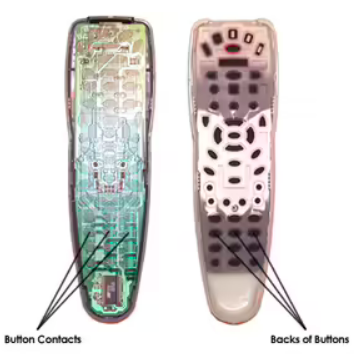
\includegraphics[width=\textwidth]{img/remotematerial1.png}%
  %\caption{KUKA's original position}%
  %\label{fig:ptp-test-orig}
\end{subfigure}
%
  \begin{subfigure}{.4\textwidth}
    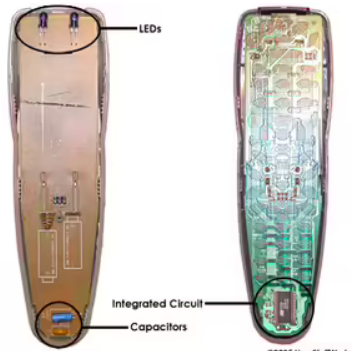
\includegraphics[width=\textwidth]{img/remotematerial2.png}%
%  \caption{KUKA's final position}%
%  \label{fig:ptp-test-final}
\end{subfigure}
%
  \caption{TV Remote control bill of materials, withdrawn from~\cite{remotematerial}}%
  \label{fig:remotemat}
\end{figure}

As can be seen in Fig.~\ref{fig:tvsells}, the amount of televisions sold per
year is about 200 million per year, with a tendency to increase over the next
years. Thus, at least the same amount of TV remotes sells is expected, as each
new TV requires one remote control, but it is expected to be exceeded due to TV
remote replacement arising from its malfunctioning or bad usage.
%
\begin{figure}[htb!]
\centering
    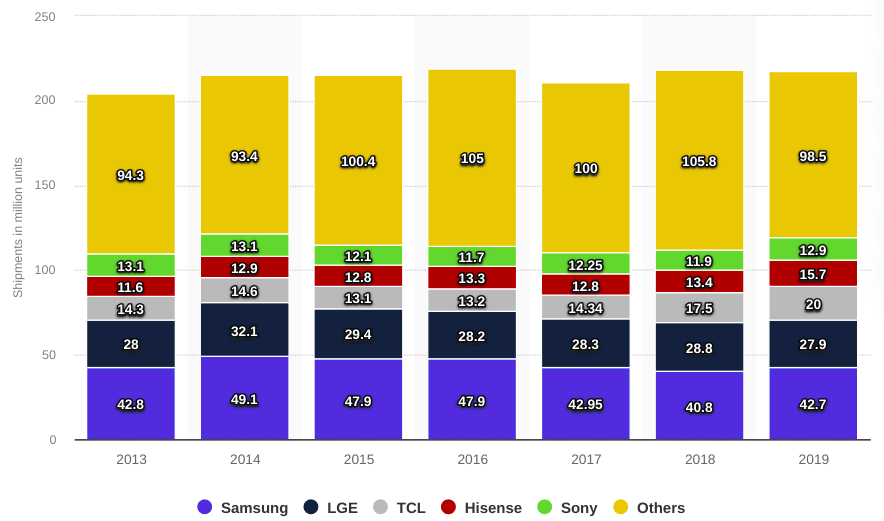
\includegraphics[width=0.7\columnwidth]{./img/tvsellings.png}
  \caption{Global LCD TV unit shipments from 2015 to 2019, by vendor (in
    millions), withdrawn from~\cite{tvsellings}}%
\label{fig:tvsells}
\end{figure}
%%% Local Variables:
%%% mode: latex
%%% TeX-master: "../../../dissertation"
%%% End:
